% Gemini theme
% https://github.com/anishathalye/gemini
\documentclass[final]{beamer}
\setbeamerfont{caption}{size=\footnotesize}

% ====================
% Packages
% ====================

\usepackage{fontspec}
\usepackage[all]{xy}
\usepackage[size=a2]{beamerposter}
\usetheme{gemini}
\usecolortheme{mit}
\usepackage{qcircuit}
\usepackage{booktabs}
\usepackage{graphicx}
  \setkeys{Gin}{width=\linewidth,totalheight=\textheight,keepaspectratio}
  \graphicspath{{graphics/}} % set of paths to search for images
\usepackage{amsmath, amssymb, physics}
\usepackage[skip=1pt, singlelinecheck=false]{subcaption}

% Inserts a Margolus target.
\newcommand{\mtarg}{*+<.02em,.02em>{\xy ="i","i"-<.39em,0em>;"i"+<.39em,0em>
**\dir{-}, "i"-<0em,.39em>;"i"+<0em,.39em>
**\dir{-},"i"*\xycircle<.4em>{}*\xycircle<.5em>{} \endxy} \qw}

% ====================
% Lengths
% ====================

% If you have N columns, choose \sepwidth and \colwidth such that
% (N+1)*\sepwidth + N*\colwidth = \paperwidth

\newlength{\sepwidth}
\newlength{\colwidth}
\setlength{\sepwidth}{0.02\paperwidth}
\setlength{\colwidth}{0.30\paperwidth}
\newcommand{\separatorcolumn}{\begin{column}{\sepwidth}\end{column}}

% ====================
% Title
% ====================

\title{On the advantages of relative phase Toffoli gates}

\author{Unathi K. Skosana \and Supervisor: Prof. Mark Tame}

\institute[shortinst]{Department of Physics, Stellenbosch University}

% ====================
% Body
% ====================

\begin{document}

    \addtobeamertemplate{headline}{} 
    {
    % \begin{tikzpicture}[remember picture,overlay, scale=0.75] 
    %     \node [shift={(-25em,-10em)}] at (current page.north east)
    %     {
\includegraphics[height=15em]{logo/logo.pdf}}; 
    % \end{tikzpicture} 
    }


    \begin{frame}[t]
        \begin{columns}[t]
            \separatorcolumn 

            \begin{column}{\colwidth}
                \begin{block}{Boolean arithmetic, universality and Toffoli gates}
                    In classical computation, the reversible \textbf{Toffoli} gate is a universal logic gate, \emph{i.e.}, any logic circuit $L$ which computes a Boolean function of the form $f: \{0,1\}^n \to \{0,1\}$ can be decomposed into a reversible logic circuit $L'$, equivalent in operation, made up of only Toffoli gates.

\begin{figure}[htpb]
    \centering
    \begin{minipage}{14pc}
        \begin{tabular}{@{}lllrlll@{}}
            \bottomrule
            \multicolumn{3}{c}{Inputs} && \multicolumn{3}{c}{Outputs} \\
            \midrule
            $a$ & $b$ & $c$ && $a'$ & $b'$ & $c'$ \\
            0 & 0 & 0 && 0 & 0 & 0 \\
            0 & 0 & 1 && 0 & 0 & 1 \\
            0 & 1 & 1 && 0 & 1 & 1 \\
            1 & 0 & 0 && 1 & 0 & 0 \\
            1 & 0 & 1 && 1 & 0 & 1 \\
            1 & 1 & 0 && 1 & 1 & 1 \\
            1 & 1 & 1 && 1 & 1 & 0 
        \end{tabular}
    \end{minipage}%
    \begin{minipage}{14pc}
        \Qcircuit @C=1.0em @R=3.5em {
            \lstick{a} & \ctrl{1} & \qw & \rstick{a'} \\
            \lstick{b} & \ctrl{1} & \qw & \rstick{b'} \\
            \lstick{c} & \targ    & \qw & \rstick{c'}
        }
    \end{minipage}
    \caption{Truth table and circuit for a Toffoli gate}
    \label{fig:toffoli}
\end{figure}
                \end{block}

                \begin{block}{Decomposition of Toffoli gates}
                    The classical Toffoli logic gate admits a realization as a unitary quantum logic gate on the merit of being reversible. As a quantum logic gate (CCX), though not universal, the Toffoli gate is a substratum for Boolean arithmetic across quantum logical registers and ensures that any classical computation is reproducible on a quantum computer
                    \begin{align}
                        \text{CCX}_{abc}: \ket{a, b, c} \mapsto \ket{a, b, c \oplus a \cdot b}.
                    \end{align}
        However, Toffoli gates are not easy to implement on current quantum hardware:
        \begin{itemize}
            \item \textbf{Not natively supported.} Current quantum hardware instead decomposes Toffoli gates onto a physically implemented (native) universal gate made up of several single qubit gates and one two-qubit gate~\cite{Barenco_1995},~\emph{i.e.}, no less than $2n$ two-qubit gates (CX, CZ, etc) for a $n$-controlled Toffoli gate~\cite{shende2008cnotcost} and the traditional three-qubit Toffoli decomposes into six CX and seven $T/T^{\dagger}$ gates:
        \begin{equation}
            \label{eq:toffoli}
            \Qcircuit @C=.5em @R=1.3em {
                & \ctrl{1} & \qw  &&&&  \qw & \qw & \qw & \ctrl{2} & \qw & \qw & \qw 
                                    & \ctrl{2} & \qw & \ctrl{1} & \gate{T} & \ctrl{1} & \qw \\ 
                & \ctrl{1} & \qw  &&& = \hspace{0.5cm} &  \qw & \ctrl{1}  & \qw & \qw & \qw 
                                    & \ctrl{1}  & \qw       & \qw & \gate{T} & \targ & \gate{T^{\dagger}}
                                    & \targ & \qw \\
                & \targ    & \qw &&&& \gate{H} & \targ & \gate{T^{\dagger}} & \targ & \gate{T}
                                    & \targ & \gate{T^{\dagger}} & \targ & \gate{T} & \gate{H} & \qw & \qw
                                    & \qw & .
            }
        \end{equation}
            \item \textbf{Decoherence.} Despite high fidelity implementations ($\gtrsim 99\%$ for superconducting qubits, see Reference \cite{Kjaergaard2020}), the effects of decoherence are considerable and set a limit on the number of two-qubit gates over a set
of qubits in a computation lest it fail.
        \end{itemize}


                \end{block}

                \begin{alertblock}{Relative phase Toffoli gates}
                    Variants of Toffoli gates, collectively called relative phase Toffoli gates, due to their operation being equivalent to that of a Toffoli gate up to some undesirable phase:

                    \begin{itemize}
                        \item \textbf{Smaller in circuit size.} Margolus gate (RCCX) is an optimal three-qubit relative phase Toffoli gate up to a relative shift ($\ket{101} \mapsto -\ket{101}$), that uses three CX gates and four single-qubit gates~\cite{Marg_1994,Song_2003}:
                    \begin{equation}
                        \label{eq:margolus}
                        \Qcircuit @C=.7em @R=.6em @!R {
                            & \ctrl{1}  & \qw &&&&                   \qw      & \qw        & \qw
                                                & \ctrl{2} & \qw      & \qw       & \qw & \qw \\
                            & \ctrl{1}  & \qw &&& = \hspace{0.5cm} & \qw      & \ctrl{1}   & \qw
                                                & \qw      & \qw      & \ctrl{1}  & \qw & \qw \\
                            & \mtarg    & \qw &&&& \gate{R_y^{+\frac{\pi}{4}}} & \targ  & \gate{R_y^{+\frac{\pi}{4}}}
                            & \targ &\gate{R_y^{-\frac{\pi}{4}}} & \targ  & \gate{R_y^{-\frac{\pi}{4}}} & \qw & .
                        }
                    \end{equation}
                    \item \textbf{Use beyond commonly conceived scenarios.} Optimization of multiply-controlled full Toffolis via relative phase Toffoli replacements~\cite{PhysRevA.93.022311}.
                    \end{itemize} 


                \end{alertblock}
            \end{column}

            \separatorcolumn

            \begin{column}{\colwidth}
                \begin{block}{Gate characterization}
                    We characterize and compare the performances of a three-qubit Toffoli gate (CCX) and Margolus gate (RCCX) in two ways on IBM's superconducting quantum processors through the Qiskit SDK~\cite{Qiskit}.

                    \heading{Via quantum state tomography}
                    We prepare an example state with a CCX in comparison to one prepared with a RCCX gate.
                    \begin{align}\label{eq:ent}
                        \ket{\psi} &= \text{CCX}_{012}\ket{1}_{0}\ket{+}_1\ket{0}_2 = \text{RCCX}_{012}\ket{1}_{0}\ket{+}_1\ket{0}_2  \nonumber, \\
                                   &= \frac{1}{\sqrt{2}}\ket{1}_0(\ket{0}_1\ket{0}_2 + \ket{1}_1\ket{1}_2) \nonumber, \\
                                   &= \ket{1}_{0}\ket{\Phi^{+}}_{12},
                    \end{align}
                    then perform state tomography on qubits $1,2$ (maximally entangled Bell state), experimentally prepared on IBM Q's seven-qubit quantum processor \textbf{ibmq\_casablanca}.

                    \begin{figure}[htpb]
                        \begin{minipage}{11pc}
                            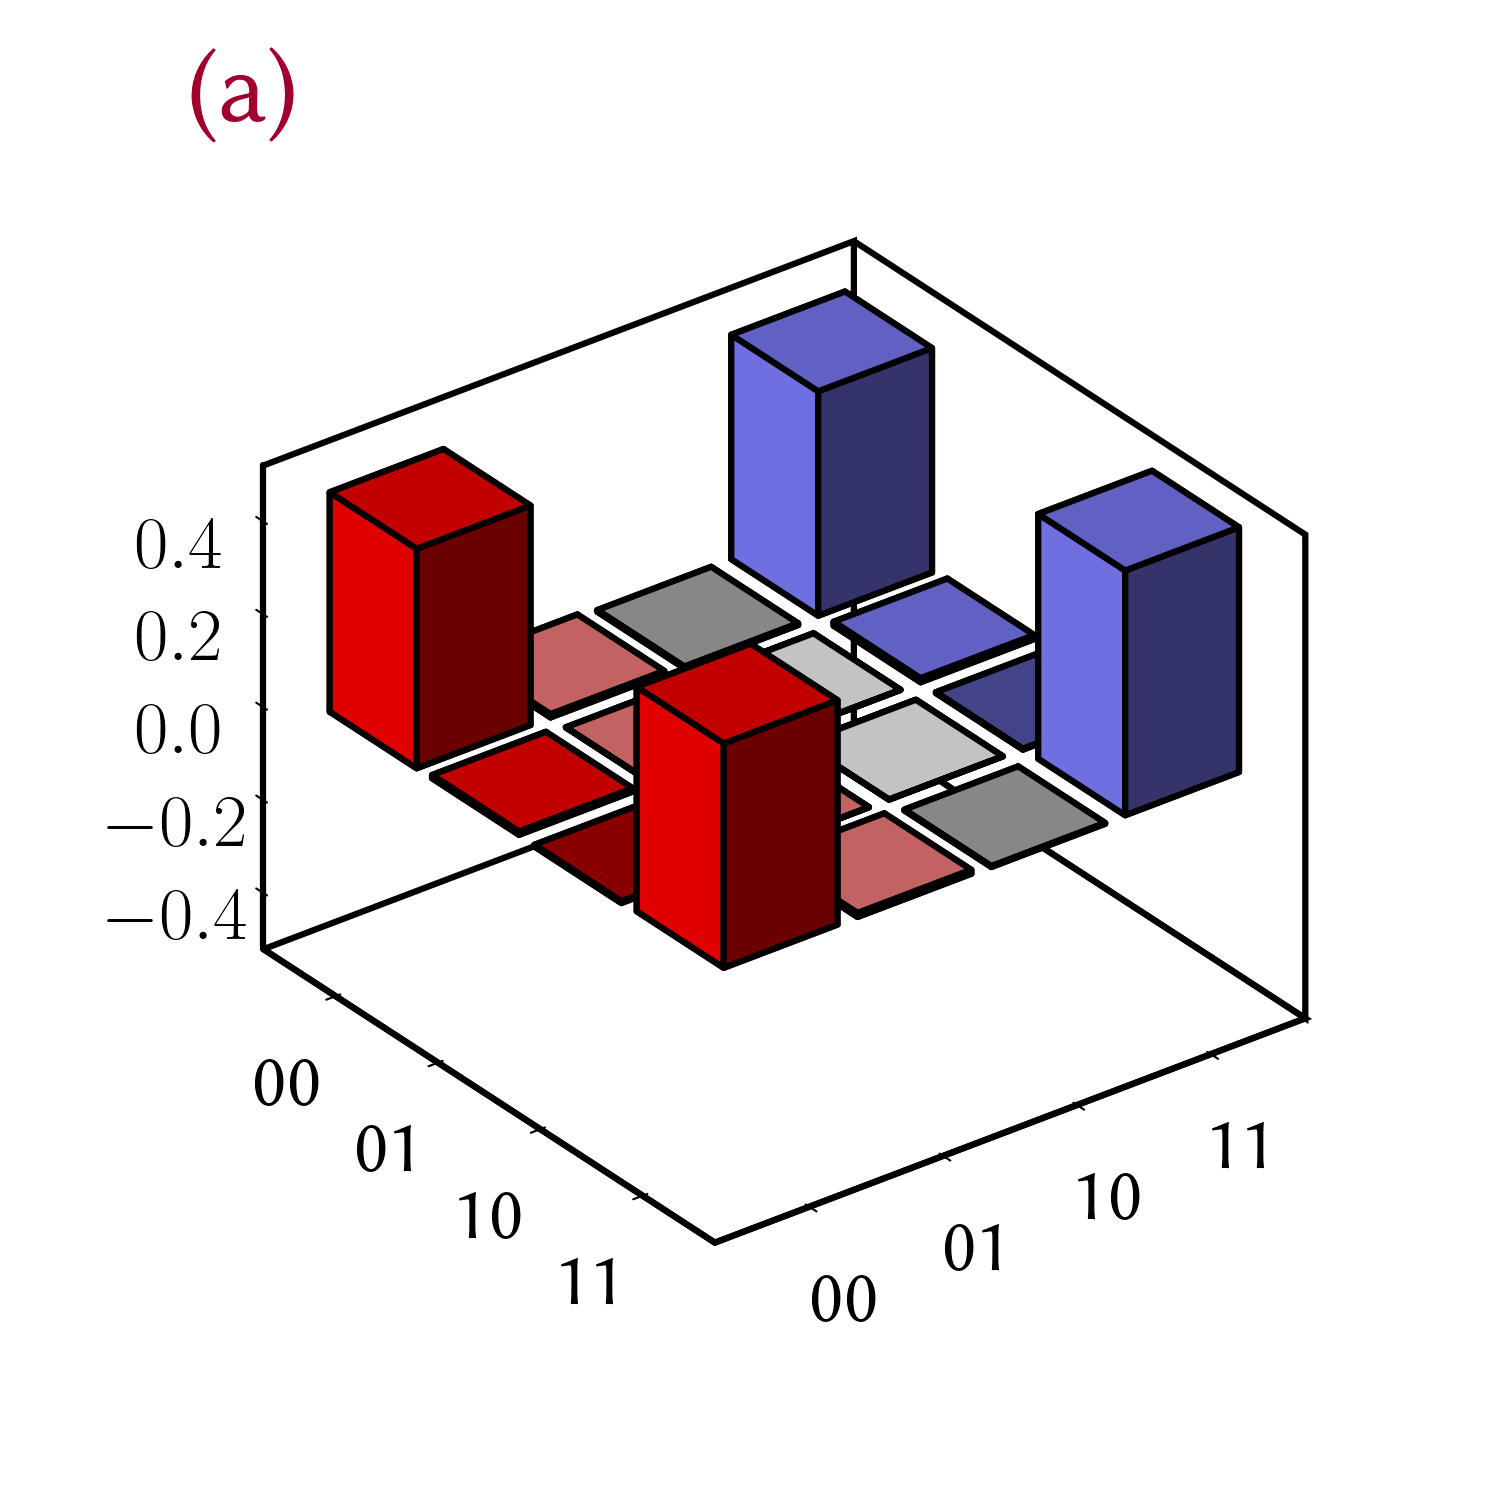
\includegraphics[width=11pc]{mat3d_toff_real.png}
                        \end{minipage}%
                        \begin{minipage}{11pc}
                            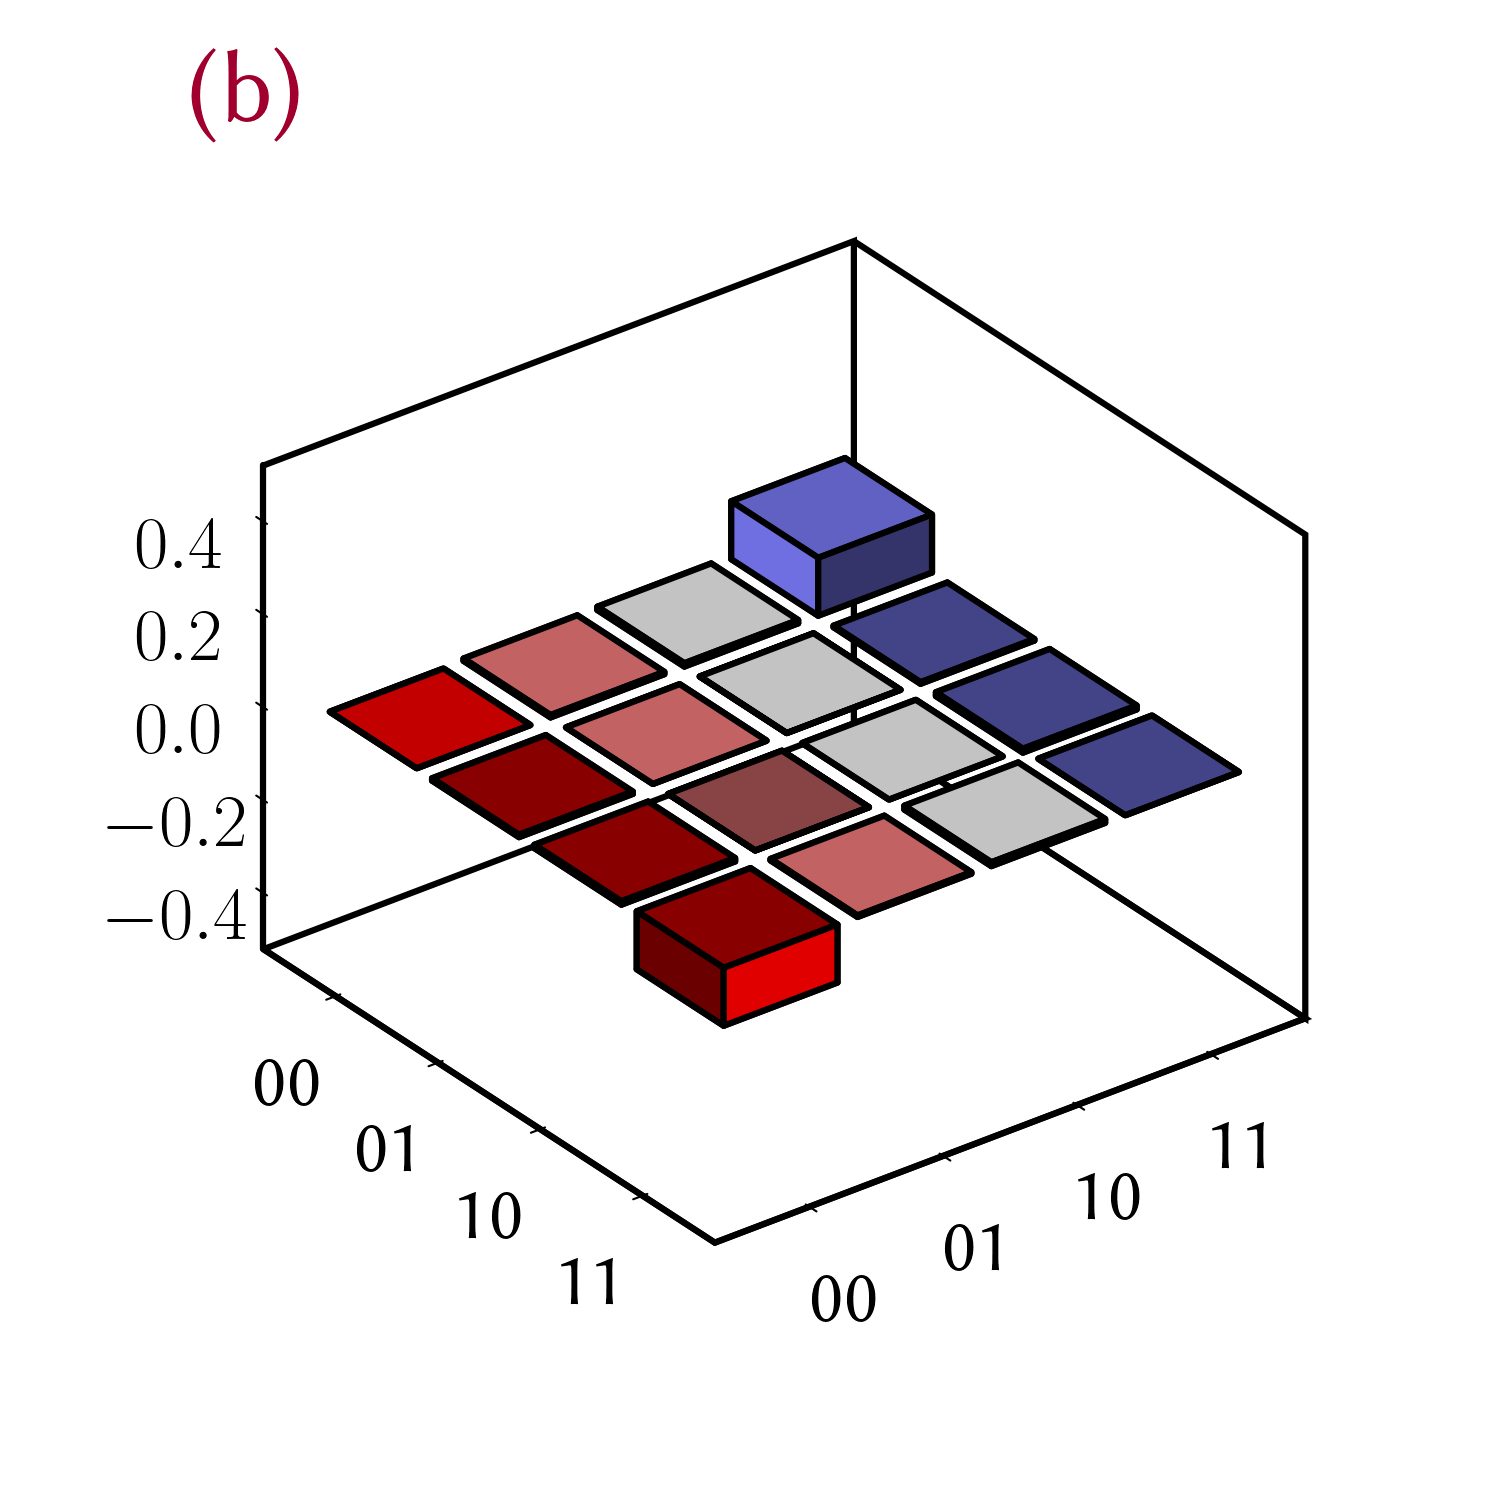
\includegraphics[width=11pc]{mat3d_toff_imaginary.png}
                        \end{minipage}%
                        \begin{minipage}{11pc}
                            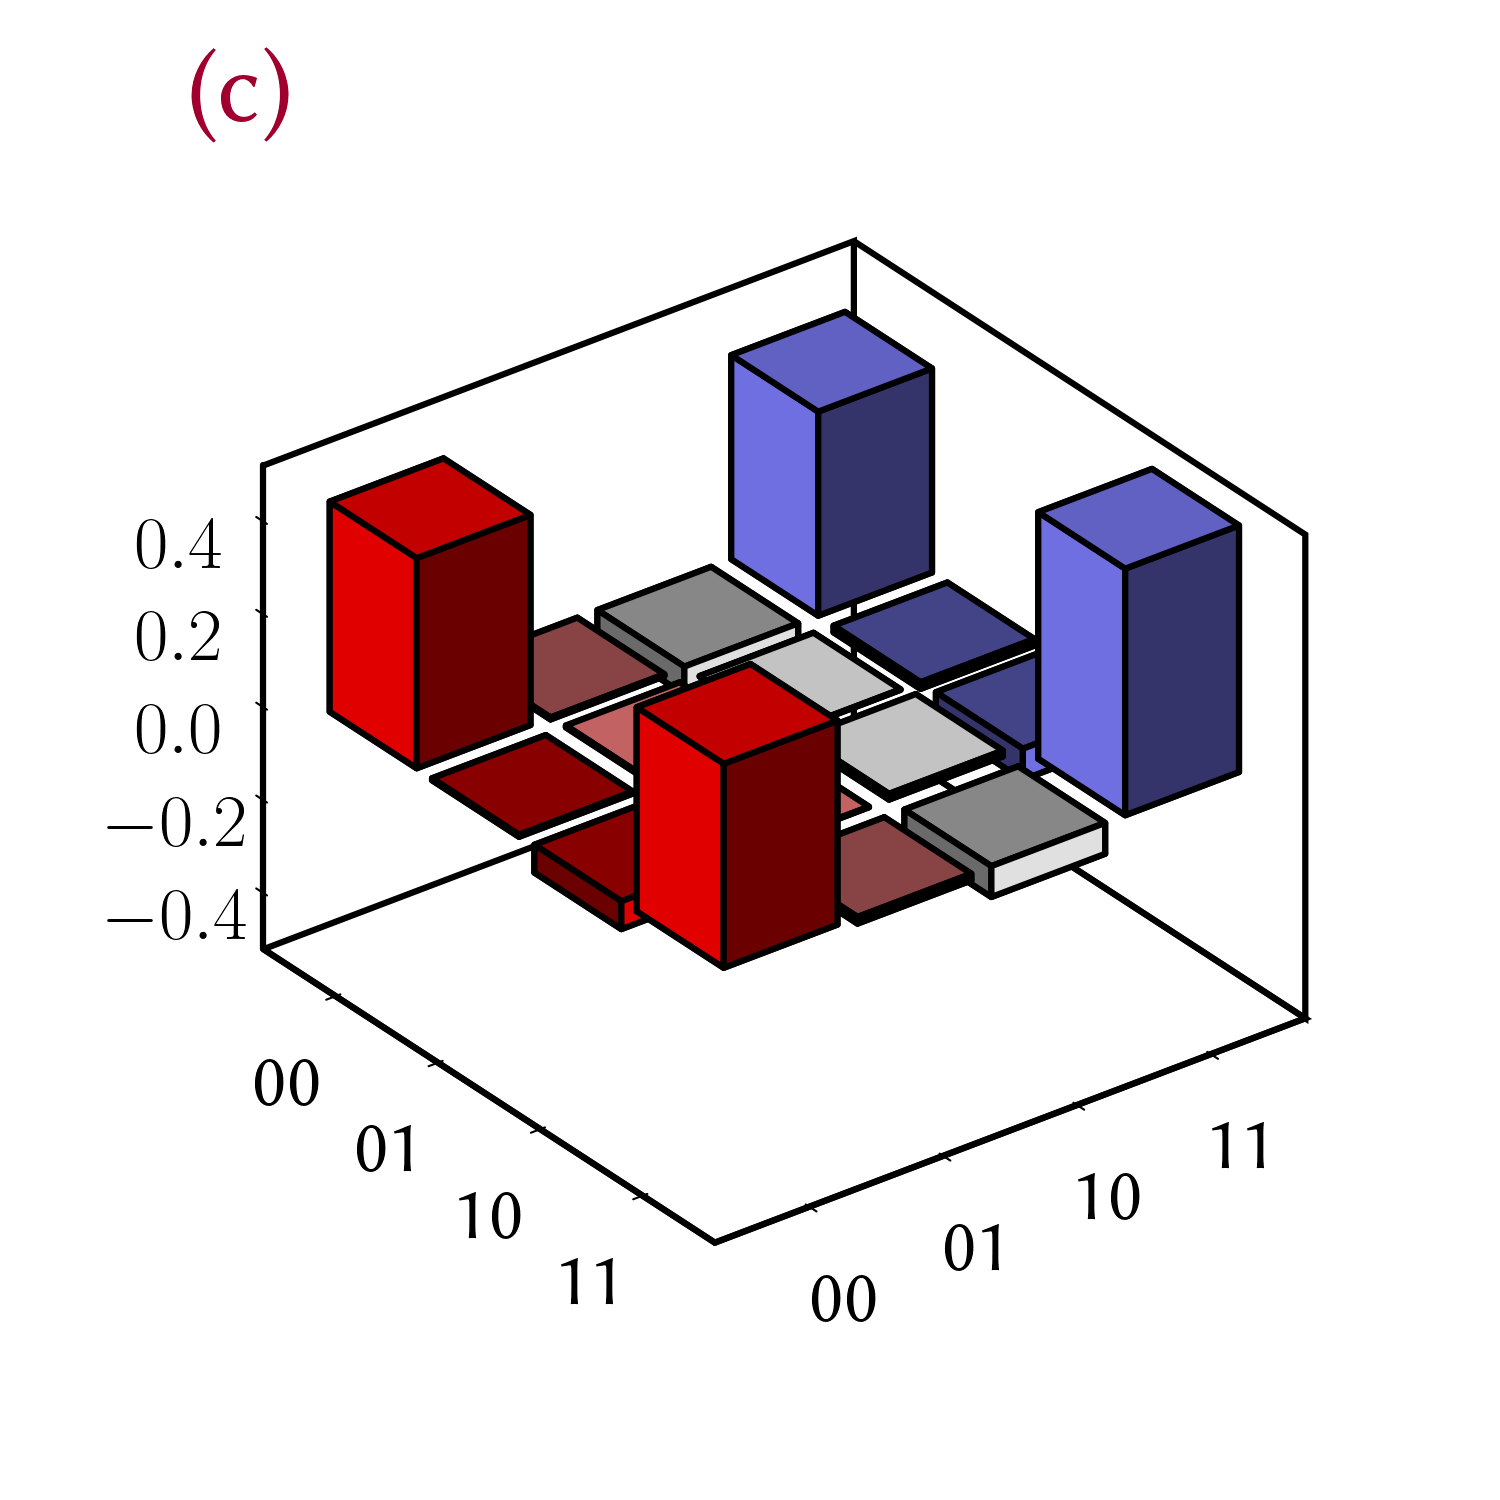
\includegraphics[width=11pc]{mat3d_rel_toff_real.png}
                        \end{minipage}%
                        \begin{minipage}{11pc}
                           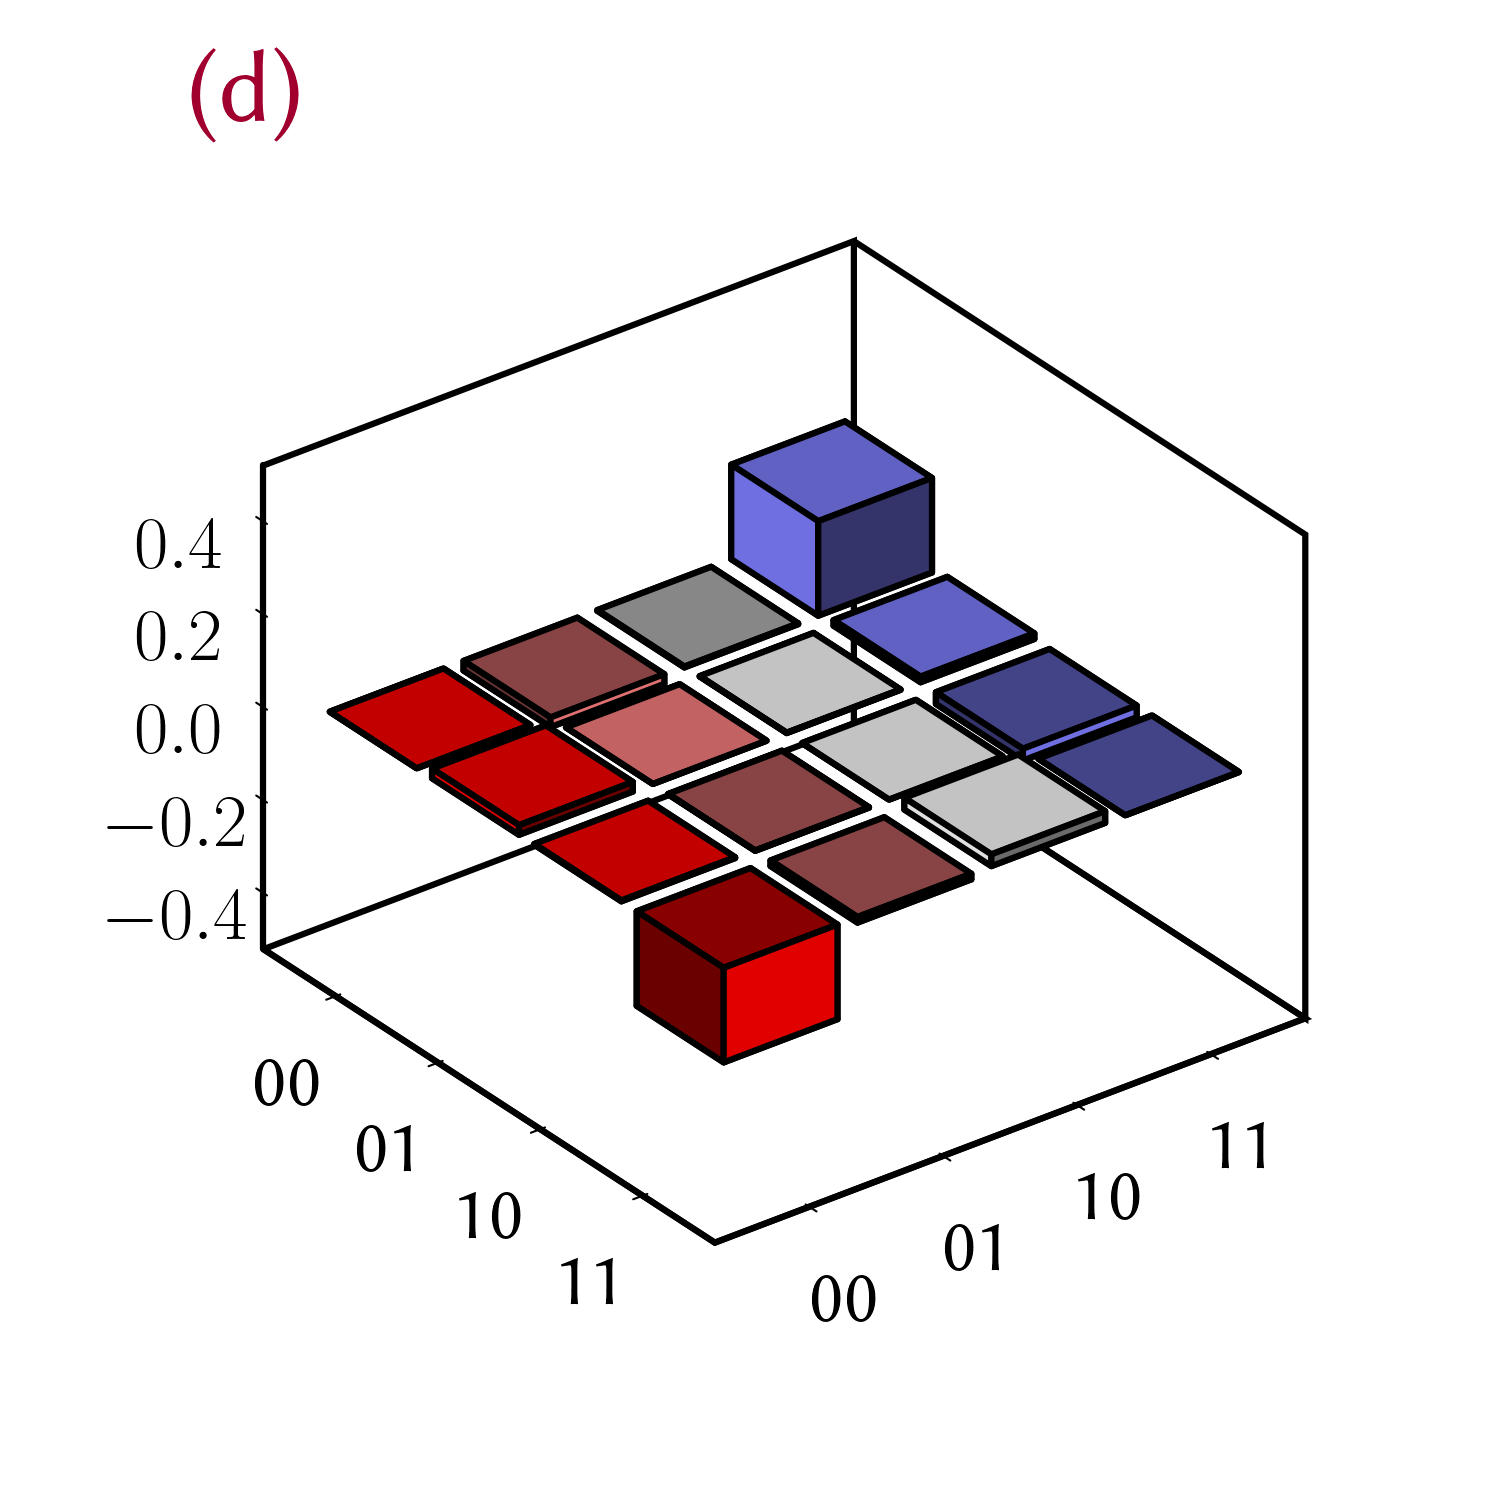
\includegraphics[width=11pc]{mat3d_rel_toff_imaginary.png}
                        \end{minipage}
                        \label{fig:mat3d}
                        \caption{(a) Real  and (b) imaginary part of the measured density matrix of the state in equation~[\ref{eq:ent}] prepared with a CCX gate on IBM Q's \emph{ibmq\_casablanca}. Similarly, (c) and (d) are real and imaginary parts, respectively, of the same state prepared with a RCCX gate.}
                    \end{figure}
                    To quantitatively evaluate the performance of the two gates in generating the Bell state in equation~[\ref{eq:ent}], we measure the fidelity for two quantum states $\rho$ and $\sigma$, defined as $F(\rho, \sigma) = \mathrm{Tr}(\sqrt{\rho^{1/2} \sigma \rho^{1/2}})$ \cite{Mike&Ike}. For this particular instance they were measured (within 95\% confidence intervals) to be $F(\op{\Phi^{+}}{\Phi^{+}}, \sigma_\text{CCX}) = 0.929 \pm 0.003$ and $F(\op{\Phi^{+}}{\Phi^{+}}, \sigma_\text{RCCX}) = 0.972 \pm 0.008$ respectively.

                    \heading{Via quantum process tomography}
                    For each a circuit, we perform process tomography and reconstruct a description of the quantum channel $\mathcal{E}$ that describes the circuit's operation on the aforesaid processor.
                    \begin{figure}[htpb]
                        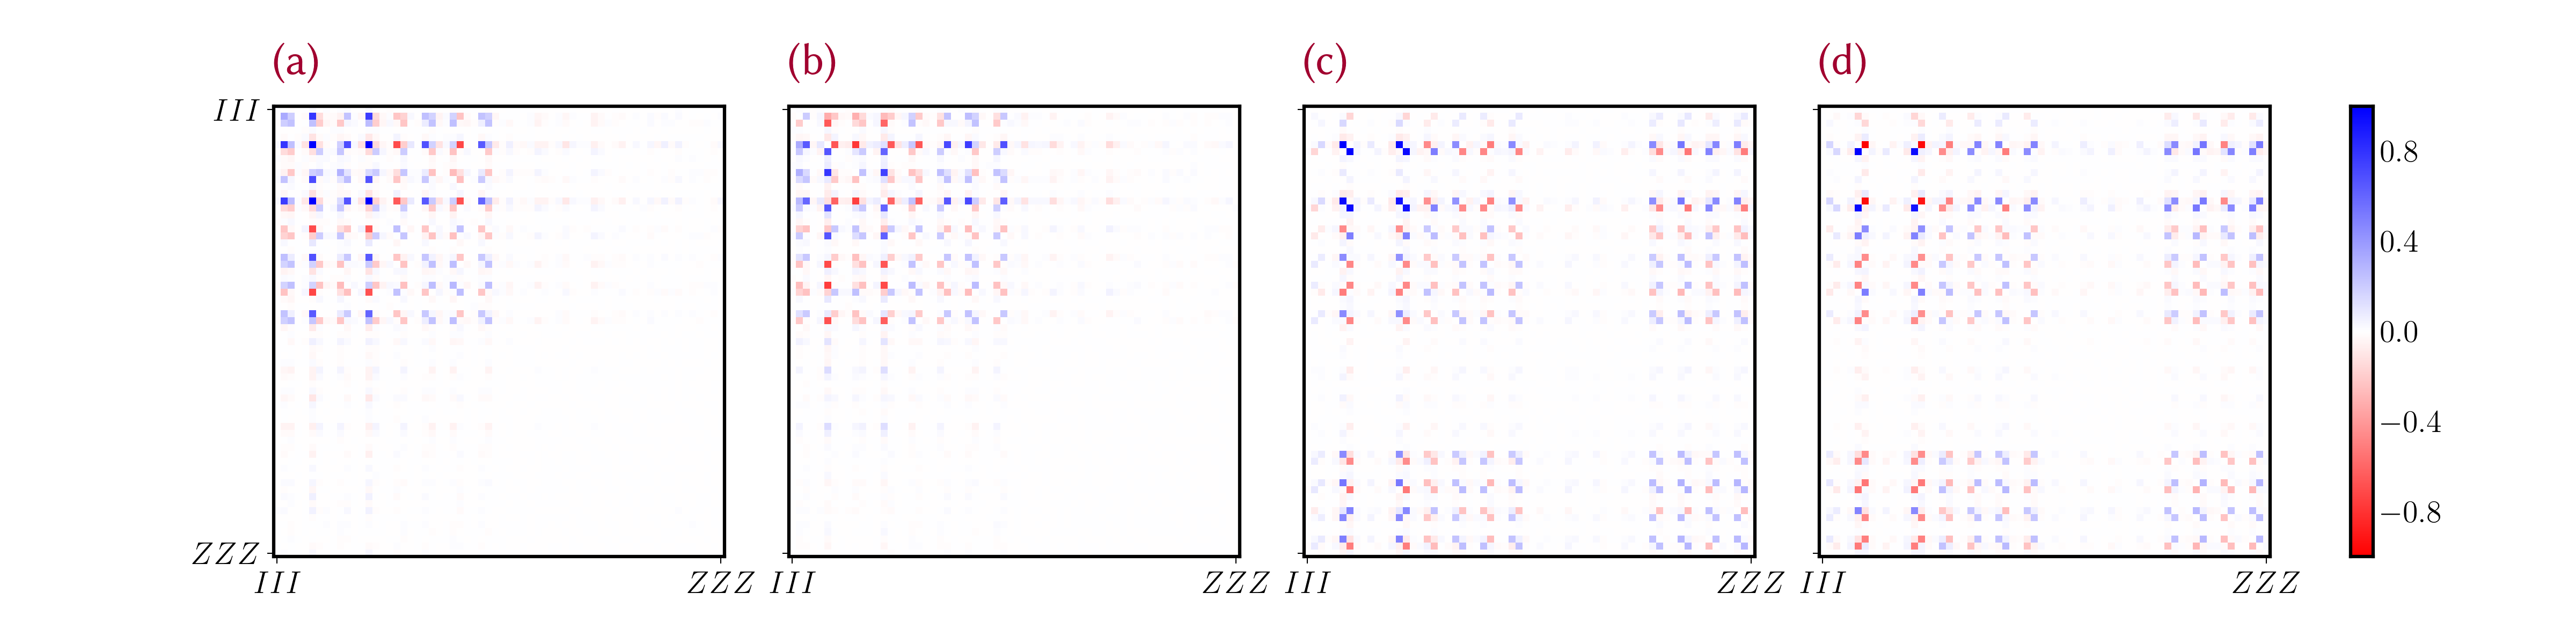
\includegraphics[width=\linewidth]{chi_mats.png}
                        \caption{(a) Real  and (b) imaginary part of the measured $\chi$-matrix representation of the quantum channel $\mathcal{E}_\text{CCX}$ prepared with a CCX gate on IBM Q's \emph{ibmq\_casablanca}. Similarly, (c) and (d) are real and imaginary parts, respectively, of the quantum channel $\mathcal{E}_\text{RCCX}$ prepared with a RCCX gate.}
                        \label{fig:mat3d}
                    \end{figure}
                 The average gate fidelity of a quantum channel $\mathcal{E}$ with respect to a target unitary $U$ measures how close $\mathcal{E}$ approximates $U$, is given by 
                 \begin{align}\label{eq:gfid}
                     & \bar{F}(\mathcal{E}, U) = \int d\psi \expval{U^{\dagger} \mathcal{E}(\dyad{\psi}) U}{\psi}, \\
                     & \mathcal{E}(\rho) = \displaystyle\sum_{i,j} \chi_{i,j} \sigma_i \rho \sigma_j \quad \text{Evolution of a density matrix $\rho$ w.r.t the $\chi$-presentation of $\mathcal{E}$.}
                 \end{align}
                 where the integration is over the uniform Haar measure and $\mathcal{E}(\cdot)$ is an evolution with respect to the quantum channel $\mathcal{E}$ (See references~\cite{Nielsen_2002,Magesan_2011} for closed forms of equation~\ref{eq:gfid}). We measured the average gate fidelities to be $\bar{F}_\text{CCX}(\mathcal{E}, U) = 0.917 \pm 0.005$ and $\bar{F}_\text{RCCX}(\mathcal{E}, U) = 0.958 \pm 0.002$ respectively.
                 \end{block}
            \end{column}

            \separatorcolumn

            \begin{column}{\colwidth}
               \begin{block}{Case studies: Quantum factoring of $N=21$}
                   In  2012~\cite{Nphoton.2012.259.10.1038}, and recently in 2019~\cite{PhysRevA.100.012305}, the integer $N=21$  was  factored,  setting  the  record  for  the  largest  integer  factored with Shor's quantum factoring algorithm~\cite{Shor_1997}.
                \begin{figure}[t]
                    \mbox{
                        \Qcircuit @C=1.0em @R=2.0em {
                            \lstick{\ket{0}} & {/} \qw & \gate{H^{\otimes n}} & \qw & \ctrl{1} & \qw &  \gate{QFT^{\dagger}} & \meter & \cw \\
                            \lstick{\ket{1}} & {/} \qw & \qw & \qw & \gate{U^x_a} & \qw & \qw & \qw & \qw
                        }
                    }
                    \caption{Schematic of the order-finding routine for Shor's algorithm for $n$ qubits. The number of qubits in the control register determines the bit-accuracy of the value of the extracted order. The bottom (work) register has the $m$ qubits required to encode $N$. First, the control and work registers are initialized, then conditional modular exponentiation is performed, indicated by the controlled unitary and an inverse quantum Fourier transform is applied to the control register followed by a standard computational basis measurement.} 
                \end{figure}
                \begin{itemize}
                    \item First scheme (Mart\'in-L\'{o}pez et al.~\cite{Nphoton.2012.259.10.1038}):
                        \begin{itemize}
                            \item \textbf{Iterative} via real-time conditionals operations and feed forward operations, recycling a single-qubit in the control register on each iteration.
                            \item \textbf{Uses full Toffolis} to implement the modular exponentiation operation.
                            \item \textbf{Full factoring not achieved,} falls one iteration short of full factorization of $N=21$.
                        \end{itemize}
                \end{itemize}

                \begin{itemize}
                    \item Second scheme (Amico et al.~\cite{PhysRevA.100.012305}):
                        \begin{itemize}
                            \item \textbf{Pseudo-iterative} via splitting the iterations into separate circuits and reseting the computation on each iteration, using a single-qubit in the work-register.
                            \item \textbf{Without the use of the continued fractions algorithm,} the order is extracted via a statistical test instead.
                            \item \textbf{Also uses full Toffolis,}  in a similar fashion to the first scheme.
                        \end{itemize}

                \end{itemize}

                \begin{itemize}
                    \item Our scheme (Skosana and Tame.~\cite{skosana2021demonstration}):
                        \begin{itemize}
                            \item \textbf{Non-iterative} uses three qubits in the control register.
                            \item  \textbf{Uses relative phase Toffolis} while preserving the functional correctness of the modular exponentiation operation.
                            \item \textbf{Fully factors} $N=21$ by giving the correct order via the continued fractions algorithm.
                            \item \textbf{Entanglement across the registers in the circuit} is verified, which is a requisite for the speed-up of the algorithm.
                        \end{itemize}
                \end{itemize}
               \end{block}

               \begin{block}{References}
                    \bibliographystyle{iopart-num}
                    \nocite{*}
                    \bibliography{poster}
               \end{block}
            \end{column}
            \separatorcolumn
        \end{columns}
    \end{frame}
\end{document}
